% Evert's latex template

\documentclass[a4paper,12pt]{article}
%\documentclass[a4paper,12pt,article]{memoir}

%% input vs include
%% input: just include everything from some external file (without intelligent processing)
%% include: renders the included file separately, gives clearpage before and after, can give speed bonus,
%% only works on one level (no nested includes are possible). includes are a good choice for book chapters.
%% When using SyncTex, you probably need to add the file extention when using input
%% (so using include is recommended for SyncTex).

%% META information
%%
%% Title, Author, Subject, Keywords
%%
%% See _pkg/hyperref.tex if you use non-ascii characters in the title or author name!!

\def \metatitle {Impressive Title Here}
\def \metadate {2016-03-14}
\def \metaauthor {Evert Mouw} % don't use comma's (,)
\def \metacontact {\url{post@evert.net}}
\def \metaorganisation {LogiStrata}
\def \metasubject {This is my subject}
\def \metakeywords {WordA WordB WordC}
\def \metaabstract {In this short paper, the main determinants of political behaviour in relation to political participation and voter turnout are discussed. Political participation is important for democracies to maintain legitimacy and quality. This participation is highly influenced by education and knowledge.}

\author{\metaauthor}
\title{\metatitle}


% packages
%% Taalondersteuning: goede woordafbreking, datumweergave, etc.
\usepackage[english]{babel}
%\usepackage[british]{babel}
% \usepackage[dutch]{babel}

%% print dates using ISO 8601 and DIN 5008 (yyyy-mm-dd)
%% language options are: english, american, german, ngerman (new german), french, ... (see doc)
\usepackage[english,iso]{isodate}
\isodate

%% Lorum Ipsum text
%% usage: \lipsum
%% or specify which paragraphs: \lipsum[4-30]
\usepackage{lipsum}

%% natbib
%% Disable when using multibb ??
%% reference sheet: http://merkel.zoneo.net/Latex/natbib.php

%% Harvard style citations.
%% Usage:
%% \citet{goossens93}  	Goossens et al. (1993)
%% \citep{goossens93} 	(Goossens et al., 1993)
%% \bibliographystyle{plainnat}  or agsm
%% http://merkel.zoneo.net/Latex/natbib.php
\usepackage[round,longnamesfirst]{natbib}

%% nice numbered system
%% broken backref: http://tex.stackexchange.com/questions/13653/hyperref-with-the-backref-page-option
%\usepackage[super,square,numbers,comma,sort&compress]{natbib}

%% meerdere bibliografieen
%% http://www.tex.ac.uk/cgi-bin/texfaq2html?label=multbib
%\usepackage{multibbl}
%% Put the code below after the \begin{document}
%\newbibliography{sources1}
%\bibliographystyle{sources1}{alpha}
%\newbibliography{sources2}
%\bibliographystyle{sources2}{plain}

%% generic math packages
\usepackage{amsmath}

%% biologische symbolen (male, female) en leadso golfpijl
%% must be loaded AFTER ams(math)
\usepackage{wasysym}

%% allows colored fonts
%% example: {\textcolor{blue}{Some text goes here.}}
%% more info: http://en.wikibooks.org/wiki/LaTeX/Colors
%% note that {Xcolor} has more possibilities for named colors than {color}
%% also consider to put these options in the document class
\usepackage{color}
\usepackage[usenames,dvipsnames,svgnames,table]{xcolor}

%% strikethrough: sout{text}
%% wavy underline: uwave{text}
\usepackage[normalem]{ulem}

%%% sta toe om bijzondere letters zoals � direct te gebruiken,
%% en dat helpt ook meteen om een foutieve woordafbreking te voorkomen
%% [uitvoer] correcte uitvoer met goede woordafbreking rond speciale tekens, met eigen CM font:
\usepackage[T1]{fontenc}
%% [invoer] correcte invoer:
%\usepackage{ucs} % unicode
\usepackage[utf8x]{inputenc} % nix=latin1, dos=cp850, win=ansinew, mac=applemac, utf8 = unicode, utf8x = unicode extended (unofficial)

%% more unicode support
\usepackage{eurosym}
\usepackage{textcomp}

%% Make litagures searchable and copyable in PDF readers
\usepackage{cmap}
%%
%% For the Linux Libertine font this is not supported, you have to use:
%\input{glyphtounicode}
%\pdfglyphtounicode{f_f}{FB00}
%\pdfglyphtounicode{f_f_i}{FB03}
%\pdfglyphtounicode{f_f_l}{FB04}
%\pdfglyphtounicode{f_i}{FB01}

%% mooier font bij pdf export: CM en EC fonts
%% !! als het goed is, wordt dit al (deels) gedaan door de \usepackage[T1]{fontenc}
%\usepackage{ae,aecompl}
%\usepackage{aeguill}
%% of gebruik PostScript fonts (niet de eerste voorkeur)
%\usepackage{pslatex}
%% or use times, palatino, newcent, bookman, libertine;
%% also, have a look at http://www.tug.dk/FontCatalogue/
%\usepackage{times}
\usepackage{tgtermes} %% Extended times: works for MikTex, and needs "apt-get install tex-gyre" for Ubuntu with Texlive
%\usepackage{libertine} %% Libertine geeft problemen met \emph of \em, zoals nesting.
%\renewcommand*\oldstylenums[1]{{\fontfamily{fxlj}\selectfont #1}} %% Alleen voor Libertine, en niet zeker of dit nodig is!

%% generic XeTeX packages
\usepackage{fontspec}
\usepackage{realscripts}
%\usepackage{xltxtra} % only for backward compatibility

% For archaic input (e.g. convert -- to en-dash)
\defaultfontfeatures{Mapping=tex-text}

%% Libertine and Inconsolata
\setmainfont{Linux Libertine O}
\setromanfont{Linux Libertine O}
\setsansfont{Linux Biolinum O}
\setmonofont{Inconsolata}

%% Liberation
%% https://en.wikipedia.org/wiki/Liberation_fonts
%\setmainfont{Liberation Serif}
%\setromanfont{Liberation Serif}
%\setsansfont{Liberation Sans}
%\setmonofont{Liberation Mono}

%% Math / Equations
%% http://tex.stackexchange.com/questions/118244/what-is-the-difference-between-unicode-math-and-mathspec
\usepackage{unicode-math} % can use both unicode chars AND descriptions for equations :-)
%%
%% choose a math font for equations
%%
%\usepackage{mathspec} % must use descriptions for equations
\setmathfont{TeX Gyre Pagella Math}
%\setmathfont{texgyrepagella-math.otf}
%\setmathfont{Latin Modern}
%\setmathfont{Asana Math}

%% use geometry OR fullpage to decrease the page margins
%\usepackage[top=2cm,bottom=2cm,left=3cm,right=2cm]{geometry}
%% sets all 4 margins to be either 1 inch or 1.5 cm, and specifies the page style.
\usepackage{fullpage}

% Make a quote environment which is italicized.
% http://tex.stackexchange.com/questions/14683/defining-environments-based-on-other-ones-whats-the-right-way
\newenvironment{italicquote}{%
  \quote
  \itshape
}{%
  \endquote
}

%% **** MEMOIR ****
%% for best formatting / layout control, swith to memoir
%% in the index.tex, change the first line to the memoir class
%% disable the fullpage above and some of the things below
%% you can use a build-in memoir theme like pedersen:
%\chapterstyle{pedersen}

%% fancy headers
%% http://texblog.wordpress.com/2007/11/07/headerfooter-in-latex-with-fancyhdr/
%% Better choice would be to switch to memoir
%%  which has a much better pagestyle support than fancyhdr and book.
%% DON'T USE FANCYHDR WITH FULLPAGE, USE GEOMETRY PACKAGE INSTEAD
%% (which adds complexity)
%\usepackage{fancyhdr}
%\pagestyle{fancy}

%% line spacing if \linespread does not suffice
%% this adds three new environments: doublespace, onehalfspace, singlespace
\usepackage{setspace}

%% suppresses widows and orphans
\widowpenalty=10000 %% prevent single line of a paragraph (called "widow") remaining on the top of the succeeding page
\clubpenalty=10000 %% prevent single line of a paragraph remaining on the bottom of the preceding page

%% vertical alignment and paragraph spacing - use either raggedbottom or flushbottom
\raggedbottom %% FIXED vertical whitespace between paragraphs, but total heigt NOT the same on all pages
%\flushbottom %% VARIABLE vertical whitespace between paragraphs, but total heigt the same on all pages

%% \frenchspacing - no extra space after a period
%% Tells LATEX not to insert more space after a period than after ordinary character.
%% This is very common in non-English languages, except bibliographies.
%% If you use \frenchspacing, the command \@ is not necessary.
%\frenchspacing

%% endnote support, for example \endnote{text here}
%% where you want the endnotes to appear, type: \theendnotes
%% This will create .ent files, sometimes errors will happen (.ent file not found)
%\usepackage{endnotes}

%% Control line space and formatting of lists (enumerate, itemize, description)
%% labelindent=\parindent, leftmargin=*, itemsep=0pt, parsep=0pt
%% The "shortlabels" option emulates enumerate-like syntax, where A, a, I, i
%% and 1 stand for \Alph*, \alph*, \Roman*, \roman* and \arabic*. This is intended mainly as
%% a sort of compatibility mode with the enumerate package, and therefore the following special
%% rule applies: if the very frst option (at any level) is not recognized as a valid key, then it will
%% be considered a label with the enumerate-like syntax.
\usepackage[shortlabels]{enumitem}
\setlist{noitemsep}

%% Discourage hyphenation
%% http://dcwww.camd.dtu.dk/~schiotz/comp/LatexTips/LatexTips.html#nohyphen
%% penalties to things that don't look nice (such as words split over two lines)
%% The default penalty for splitting a word is rather low.
%% Increasing penalty will produce lines with a little more extra spacing between words,
%% and you should therefore increase TeX's tolerance for such lines.
%% adjusting \tolerance appears to be most promising
%% A \hyphenpenalty of 10000 (almost) prevents hyphenation, but produces overlong and/or ugly lines.
%\hyphenpenalty=5000
%\tolerance=1000

%% insert a pagebreak before a section
%% Gabriel Many, 2008-08
%% Evert Mouw, 2009-01
\makeatletter
\renewcommand{\section}{\@startsection
{section}
{1}
{0mm}
{-3.5ex \@plus -1ex \@minus -.2ex}
{2.3ex \@plus.2ex}
{\clearpage\phantomsection\normalfont\Large\bfseries}}
\makeatother{}

%% These two commands increase the space between two paragraphs
%% while setting the paragraph indent to zero.
%% but...
%% "parskip should not be used as it will also modify settings for 
%% list environments, table of contents, etc., and headings."
%% (An essential guide to LATEX2e usage - Obsolete commands and packages)
\setlength{\parindent}{0pt}
\setlength{\parskip}{1ex plus 0.5ex minus 0.2ex}

%% Elegant section numbering
%%
%% Pascal de Bruijn - The p-Code Machine - LaTeX tips & tricks
%% Source: http://blog.pcode.nl/2007/07/19/latex-tips-tricks/
%%
%% Modified by Evert Mouw to
%% - prefix the section symbol \S
%% - make it Gray; needs \usepackage[usenames,dvipsnames]{color}
%%
%% For my thesis I wanted the section numbering to be visible in the margins. This way the section titles
%% would be %% nicely lined up with my text, producing a very elegant look. Here is how you can do it:
\usepackage{sectsty}
\makeatletter\def\@seccntformat#1{\protect\makebox[0pt][r]{\textcolor{Gray}{\S \csname the#1\endcsname}\hspace{12pt}}}\makeatother

%% code listing and verbatim
\usepackage{listings}
\lstset{
breaklines=true,
breakautoindent=true,
frame=single,
basicstyle=\ttfamily,
keywordstyle=\color{OliveGreen},
commentstyle=\color{Gray},
numbers=left,
stepnumber=1,
numbersep=5pt,
numberstyle=\tiny\color{Melon}
}
%% use example:
%%\begin{scriptsize}
%%\lstinputlisting[language=VBscript]{mergenoses.bas}
%%\end{scriptsize}
%% or:
%% \begin{lstlisting}
%% put your code here
%% \end{lstlisting}

%% If you are using the hyperref (below), you don't need to load url
%% because it already provides the \url{...} command.
% \usepackage{url}

%% HYPERREF for better URLs, internal references, PDF properties, ...
%% Make sure it comes last of your loaded packages, to give it a fighting chance
%% of not being over-written, since its job is to redefine many LATEX commands.
%% Some interesting options:
%% [bookmarks] a set of PDF bookmarks will be created
%% [bookmarksopen] expand all the PDF bookmark subtrees
%% [hyperindex] attempts to make items in the index by hyperlinked back to the text
%% [unicode] you can use unicode characters in bookmarks
%% [breaklinks] allow links to break over lines
%% [hidelinks] gives you active links in black without a box around them
%% backreferences: DO CURRENTLY NOT WORK, DUNNO WHY NOT!!!!!!!!!!!!!!!!!!!!!!!!!!!!!!
%% [backref] inserts extra back links into the bibliography for each entry,
%%  optional values are: section, slide, page, none, or false. If no value is given, section is taken as default.
%%
%% Backend driver if not specified: pdftex / xetex (autodetection),
%% or specify a driver using a package option...
\usepackage[bookmarks,bookmarksopen,breaklinks,hyperindex,unicode,backref=page]{hyperref}

%% PDF properties using package hyperref
%% Note: hyperref pdfusetitle option does not allow for non-ascii chars
\hypersetup{pdftitle={\metatitle}}
\hypersetup{pdfauthor={\metaauthor}} % don't use comma's (,)
\hypersetup{pdfsubject={\metasubject}}
\hypersetup{pdfkeywords={\metakeywords}} % normally seperated by comma's (,)
\hypersetup{pdfstartview={FitH}}
\hypersetup{pdfpagelayout={OneColumn}}

%% colored links inside the document
%% http://en.wikibooks.org/wiki/LaTeX/Packages/Hyperref
%% you can use, for example: black, red, green, cyan, magenta, blue
\hypersetup{colorlinks=true} % color frames (false) or colors the text of the links (true)
\hypersetup{linkcolor=blue} % color of internal links (sections, pages, etc.)
\hypersetup{citecolor=blue} % color of citation links (bibliography)
\hypersetup{filecolor=magenta} % color of file links
\hypersetup{urlcolor=magenta} % color of URL links (mail, web)

%% backreferences formatting
%\usepackage[backref]{backref}
%% alternate colors: http://en.wikibooks.org/wiki/LaTeX/Colors
%% leadsto: Not predefined in LATEX2e. Use one of the packages latexsym, amsfonts, amssymb, or wasysym. See _pkg/font.tex
\renewcommand*{\backref}[1]{}% for backref < 1.33 necessary
\renewcommand*{\backrefalt}[4]{%
\ifcase #1 %
\textcolor{CornflowerBlue}{$\leadsto$ No citations.}%
\or
\textcolor{CornflowerBlue}{$\leadsto$ Cited on page #2.}%
\else
\textcolor{CornflowerBlue}{$\leadsto$ Cited #1 times on pages #2.}%
\fi
}

%% fixes links to tables or figures which point to the caption beneath the table or figure
%% must be loaded after the hyperref package
%% DO NOT USE when using the "caption" package, because that package already
%% has it's own solution build-in and the hypcap package breaks that
%% THE CAPTION PACKAGE IS PREFERRED!!
%\usepackage[all]{hypcap}

%% Different font in captions under tables and figures (METHOD 1, PREFERRED)
%% also, has the functionality of "hypcap" (fixes links to tables or figures
%% which point to the caption beneath the table or figure) build-in, DO NOT LOAD hypcap
%% CAPTION MUST BE LOADED BEFORE SUBFIG (subfig includes caption but sets no options)
\usepackage[font=small,format=plain,width=.8\textwidth,labelfont=bf,up,textfont=it,up,hypcap=true]{caption}

%% Different font in captions under tables and figures
%% Change the first line to choose another font change.
%% http://dcwww.camd.dtu.dk/~schiotz/comp/LatexTips/LatexTips.html#captfont
%\newcommand{\captionfonts}{\small}
%\makeatletter  % Allow the use of @ in command names
%\long\def\@makecaption#1#2{%
%  \vskip\abovecaptionskip
%  \sbox\@tempboxa{{\captionfonts #1: #2}}%
%  \ifdim \wd\@tempboxa >\hsize
%    {\captionfonts #1: #2\par}
%  \else
%    \hbox to\hsize{\hfil\box\@tempboxa\hfil}%
%  \fi
%  \vskip\belowcaptionskip}
%\makeatother   % Cancel the effect of \makeatletter{}

%% when picture files are in a subdirectory,
%% then specify their path using:
%% \graphicspath{{_example/}}

%% let op graphicS is verouderd
%% dit pas laden na de pst tricks
%% package opties o.a. pdftex, xetex (probeer eerst autodetect, dus geen optie)
\usepackage{graphicx}

%% prevent floats from crossing a section
%% (from Chapter 5 of LaTeX Beginner's Guide by Stefan Kottwitz)
\usepackage[section]{placeins}

%% precise image positioning with the float package
%% \begin{figure}[H]
%% the H specifier places the float at precisely the location in the LaTeX code
\usepackage{float}
\restylefloat{figure}
\restylefloat{table}

%% afbeeldingen floating maken (wrapfig) en naast elkaar zetten (subfig)
\usepackage{wrapfig}
%\usepackage{placeins} % activated  before (see above)
\usepackage{subfig}

%% improved footnote presentation
%% alas, the hyperref support will not work any more
%% see texlive bug #533602 http://bugs.debian.org/cgi-bin/bugreport.cgi?bug=533602
%% so load this AFTER the hyperref package, so we can disable hyperfootnotes
\hypersetup{hyperfootnotes=false} % but generates a warning: Option `hyperfootnotes' has already been used, (hyperref) setting the option has no effect
\usepackage[bottom,multiple,hang]{footmisc}

%% todo items
%% \todo{Something to do yet \ldots} % sidenote (margin note)
%% \todo[inline]{Some paragraph or figure caption yet to write \ldots}
%% \missingfigure{Draw some figure here.}
%% \listoftodos % create a list of to-do's
%% options:
%% dutch - use dutch text strings (english is default; for other languages, see the docs)
\usepackage{todonotes}

%% (is compatible with the hyperref package)
%% The minitoc package is useful to add mini-tables-of-contents (minitocs)
%% at the beginning of every chapter. They are also minilofs and minilots.
%% At the part level, they are parttocs, partlofs and partlots.
%% If the type of document does not use chapters, they are
%% section level secttocs, sectlofs and sectlots.
\usepackage{minitoc}

\usepackage{boxedminipage}

\newcounter{textbox}
\newenvironment{textbox}[1]%
{
	\refstepcounter{textbox}%
	\par%
	\medskip%
	\noindent%
	\textbf{Textbox~\thetextbox: #1}%
	\\%
	\medskip%
	%\begin{center}%
	\begin{boxedminipage}{\textwidth}%
	\rmfamily{}%
}
{
	%\end{center}%
	\end{boxedminipage}%
	\medskip{}%
}

%% Table stuff

%% rotate table headers by using one of these methods:
%% - \begin{sidewaystable} (needs the rotate package)
%% - rotatebox{degrees}{text} (needs the graphicx package)

%% for auto-width text-wrapped colums in tables, the X is auto-width
%% example: \begin{tabularx}{\textwidth}{ X l l l l l l l }
\usepackage{tabularx}

%% Rotating
%%
%% Pascal de Bruijn - The p-Code Machine - LaTeX tips & tricks
%% Source: http://blog.pcode.nl/2007/07/19/latex-tips-tricks/
%%
%%  Every once in a while your tables get to wide to fit on a portrait A4 page.
%% Don’t panic, the rotating package will come to the rescue.
%% Using the sideways environment (defined by the rotating package) you can rotate
%% an object (a table for example) 270/90 degrees.
%% Please note that only the object is rotated. This means page headers and footers
%% remain as they were, not disrupting the document flow.
%%
%% sidewaystable --> for table
%% sidewaysfigure --> for figure
%% sideways --> for everything

%\usepackage{rotating}
%%
%% Example of use:
%%
%\begin{sideways}
% % thing to rotate comes here
%\end{sideways}



% Clever reference must be the last one
\usepackage{cleveref}
\crefname{textbox}{textbox}{textboxes}
\Crefname{textbox}{Textbox}{Textboxes}

\begin{document} \let\ref\cref

\phantomsection
\addcontentsline{toc}{section}{Front page}

\pagenumbering{arabic}
\thispagestyle{empty} % op de eerste pagina geen paginanummer

\addvspace{40mm}

\begin{center}
%% alternate colors: http://en.wikibooks.org/wiki/LaTeX/Colors
\textcolor{OrangeRed}{printed on \today}\\
\bigskip
\huge{\metatitle}
\end{center}

\begin{figure}[H]
	\centering
	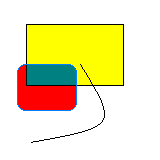
\includegraphics[scale=1.0]{_example/AFBEELDING.png}
	\caption{BESCHRIJVING VAN AFBEELDING}
	\label{fig:AFBEELDING}
	\todo[inline]{Hier nog een afbeelding toevoegen etc.}
\end{figure}

\addvspace{40mm}

\begin{abstract}
\noindent{\metaabstract}
\end{abstract}

\addvspace{40mm}

\begin{tabular}{l l}
\textit{Author}			&	\metaauthor \space <\metacontact> \\
\textit{Date}			&	\metadate \\
\textit{Institution}	&	\metaorganisation \\
\textit{Subject}		&	\metasubject \\
\textit{Keywords}		&	\metakeywords \\
\end{tabular}

\clearpage

\section*{ToDo}
This is an example latex file created by Evert. Don't forget a few things (see the todo).
\todo[inline]{Update the frontpage: frontpage.tex}
\todo[inline]{Update the metadata: meta.tex}
\bigskip
\listoftodos
\clearpage

\tableofcontents
\clearpage

%\linespread{1.3}
\onehalfspace

\graphicspath{{_example/}}

\noindent
\textit{Just a few random pieces of text (latex) I wrote when I was still a student.}

\section{The importance of political behaviour}

\todo{Create an introduction}

\begin{quote}
\textit{The most serious political problems tend to arise over the collective production of goods that are also collectively consumed.} \citep[p. 34]{laver}
\end{quote}

\noindent
Rational individuals do not contribute to collective goods. They rather take a free ride, reaping the collective benefits without costs because they can not be excluded from a public good. If all individuals in the group are rational, then no one will contribute to the public good, and the realisation of the collective good will be hopeless. This collective action problem is best illustrated in the story of the "Tragedy of the Commons". A bunch of farmers have a common ground where sheep can pasture. If too many sheep graze, than the pasture will become over-grazed. But each individual farmer should add a few extra sheep on the pasture to maximize his profit, because the disadvantages from overgrazing will be shared by all. It is easy to see how this works out without some Hobbesian outsider who enforces rules to protect the pasture. \citep[p. 36, 48-50]{laver}

\ldots

Voter turnout of young adults is often low. \citet{plutzer} offers a developmental framework to understand turnout. In short, he distinguishes two kinds of citizens: habitual voters and habitual nonvoters. Both display inertia: becoming a voter needs some trigger, and vice versa. Education is an important tool to transform nonvoters in voters. \citeauthor{plutzer} regards age and development (education) as starting variables. Becoming a civic active citizen is a path-dependent process. One starts as a young nonvoter, and peer groups consists of other nonvoters. As one ages, one gets educated, married, a home owner and so on, one gets more incentives to vote and one gets more political knowledge. Once the inertia is overcome, a nonvoter becomes a voter and often (thanks to inertia) does not change back. The speed of this development can be increased by better political education and more participation to social groups and associations.

Cited: \cite{laver,plutzer}

\section{subfig}

\begin{figure}[h]
	\centering
	\subfloat[gebit foto 1]{
		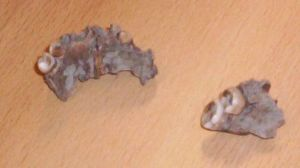
\includegraphics[scale=0.7]{gebit1.jpg}
	}
	\qquad
	\subfloat[gebit foto 2]{
		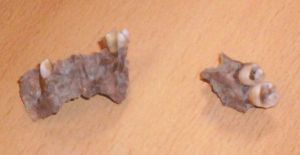
\includegraphics[scale=0.7]{gebit2.jpg}
	}
	\caption{Maxilla.}
	\label{fig:sk3_gebitten}
\end{figure}

Hier heeft \cite{laver} niets mee van doen.

\section{wrapfig}

\begin{wrapfigure}{R}{0pt}
	\centering
	%\begin{center}
		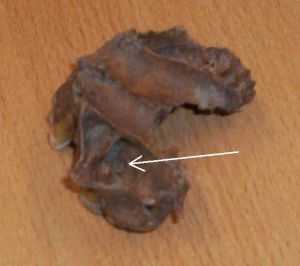
\includegraphics[width=0.6\textwidth]{fistel1.jpg}
	%\end{center}
	\caption{Fistel naar de sinus maxillaris.}
	\label{fig:fistel}
\end{wrapfigure}

\lipsum[1-3]

\section{Formatting}

Gebruik \emph{emph} en niet \emph{textit} omdat \emph{textit} niet kan nesten.
Bovendien is \emph{emph} semantisch en kan de opmaak ervan nog gewijzigd worden.
Zie ook \url{http://tex.stackexchange.com/questions/1980/emph-or-textit}

\begin{textbox}{Dit is een tekstbox}
\label{text:somename}
The actual text comes here.

Do you like it?
\end{textbox}

\subsection{Litagures -- try copy and paste}

ff fi fj fl ffi ffl ffj

\subsection{font stuff}

\sout{strikethrough},
\uwave{underwave},
\underline{underline},
\textcolor{red}{red},
\textcolor{OrangeRed}{OrangeRed},
\textsc{SmallCaps},
\texttt{TypeWriter},
\textit{Italics},
\textsl{Slanted},
\textbf{Bold},
\emph{Emphasis}

\subsection{unicode}

Does this work? Also copying and pasting to a text editor?

02 - comma's are `nice' \\
03 - euro € \\
04 - often used @ ! ( { [ ] } ) ~ \\
05 - commercial © ® ™ \\
06 - special ‘’‚‛“”„ comma \\
07 - funny ☺☻☼♠♣♥♦♫ \\
08 - gender ♂♀ \\
09 - math ≈≠≡≤√≥⅔₧ \\
10 - western ßæçèéëîñõø \\
11 - pi π \\
99 - runes ᚱᚢᚾᛖᛋ

Runes with the specific Hnias font, method 1 (newfontface):

\newfontface{\runes}{Hnias}
{\runes ᚱᚢᚾᛖᛋ}

Runes with the specific Hnias font, method 2 (xetex only):

%% XETEX Only!!
%% custom font, using a .ttf or .otf file
\setmainfont[Path=_example/]{Hnias31_runes.ttf}
%% set back to main font as specified in font_xetex.tex
ᚱᚢᚾᛖᛋ
\setmainfont{Linux Libertine O}

\section{Lijstjes}

\subsection{enumerate}

Bij de wervelkolom zijn diverse aandoeningen aanwezig:
\begin{enumerate}[I.] % I --> roman numbers, see formatting.tex in _PKG
\item Scoliose is vooral lumbaal goed zichtbaar bij de overgang naar het sacrum.
\item De spondylolyse op wervel L3 is terug te voeren op een mechanisch trauma. De wervelboog is afgebroken door teveel aanspanning (overbelasting) van de rugspieren. Hetzelfde euvel is ook bekend bij eskimo's die in kayaks hun rugspieren flink gebruiken, en bij mensen aan het begin van de vorige eeuw die tewerkgesteld werden en plots zware lichamelijke arbeid moesten verrichten waar ze niet aan gewend waren.
\item Beginnende DDD is vooral hoog lumbaal en laag thoracaal zichtbaar. Er zijn forse Schmorlse noduli.
\end{enumerate}

\subsection{description}

\begin{description}[style=sameline,leftmargin=3cm] % the options are from the enumitem package
\item[Data users] such as the departments of radiology and psychiatry.
\item[ADICT] the IT department of the AMC, also responsible for the IT security policy of the AMC.
\item[Ethical Board] of the AMC which might offer opinions and facts about patient privacy
\end{description}

\subsection{itemize}

Using interviews has also a number of drawbacks:
\begin{itemize}
\item The interpretation of interviews is very subjective.
\item Subjects could be restricted because anonymization is nearly impossible.
\item Organizational (political) sensitivities could be triggered.
\end{itemize}

\subsection{table}

\begin{table}\footnotesize
	\centering
	\begin{tabularx}{\textwidth}{ X l l l l l l l }
		&\rotatebox{90}{Jean Herveg}	&\rotatebox{90}{Corette Ploem}	&\rotatebox{90}{Heleen Dupuis}	&\rotatebox{90}{Bart van der Sloot}	&\rotatebox{90}{Beer Franken}	&\rotatebox{90}{Neugrid}	&\rotatebox{90}{MEAN}\\
	\hline \\
	Is informed consent needed?	&+	&+	&+	&+[4]	&+	&+	&+\\
	 $\backslash$-- If yes, must it be written consent?	&?	&+	&?	&?	&?	&+	&+\\
	 $\backslash$-- If yes, must it be specific for each research?	&+	&-[2]	&+	&+	&?	&+	&+\\
	Is genetic data medical data or (also) identifiable and personal data?	&+	&+	&+	&+	&+	&+	&+\\
	Is it allowed to use distributed computing?	&+[1]	&?	&+	&?	&?	&+	&+\\
	 $\backslash$-- If it is, is it also allowed to process facial images and genetic data?	&?	&?	&-	&-	&-	&+	&-\\
	Must a contract between all involved into the distributed resources be present?	&?	&?	&+	&?	&+	&?	&+\\
	Could distributed computing be used for patient care such as diagnosis or treatment (non-research)?	&?	&?	&+[3]	&+		&-&?	&?\\
	\hline \\
	\end{tabularx}
	\noindent
	+ = yes, - = no, ? = unknown or missing
	\begin{enumerate}
		\item yes, but maybe current security measures are not strong enough
		\item a broad consent for the use of tissue is practical, but for each specific research a new ethical review is necessary
		\item yes, but only if all data is encrypted
		\item but informed consent is outdated and problematic (see interview)
	\end{enumerate}
	\caption{Opinions of experts}
	\label{expertopinions}
\end{table}

\begin{table}[H]
	\centering
	\begin{tabular}{ l l l }
		Fruit	&Price	&Taste\\
		\hline \\
		Oragne	&5	&Nice\\
		Apple	&6	&Good\\
	\end{tabular}
	\caption{Fruits.}
	\label{fruits}
\end{table}

\section{Equations}

Math modes

$a+b=\int_{\xi}^{\theta} f(x)\,dx$

$a+b=∫_ξ^θ f(x)\,dx$

\section{Author}

\begin{wrapfigure}{l}{0pt}
	%\begin{center}
		
\includegraphics[width=30pt]{evert.jpg}
	%\end{center}
\end{wrapfigure}

\paragraph{Evert Mouw}
\textit{studeerde politicologie en medische informatica}\\
Email: post@evert.net

\paragraph{Barge's Anthropologica} houdt zich bezig met wetenschappelijk onderzoek en onderwijs op het gebied van fysische antropologie. Het centrum is verbonden aan het Leids Universitair Medisch Centrum. Dit verslag is tot stand gekomen als onderdeel van een studieopdracht tijdens de zomercursus voor studenten in 2007. Meer informatie over het centrum is te vinden op \url{http://www.bargesanthropologica.nl/}.


%% UNDO insert a pagebreak before a section
%% Gabriel Many, 2008-08
%\makeatletter
%\renewcommand{\section}{\@startsection
%{section}
%{1}
%{0mm}
%{-3.5ex \@plus -1ex \@minus -.2ex}
%{2.3ex \@plus.2ex}
%{\normalfont\Large\bfseries}}
%\makeatother

%% backreferences: see _pkg/hyperref.tex

\clearpage
\phantomsection
\addcontentsline{toc}{section}{References}
%\bibliographystyle{plain}
%\bibliographystyle{alpha}
\bibliographystyle{_pkg/apsr-url} % use apsr-url for political science (_pkg/apsr-url.bst needed)
%\nocite{*} % shows all entries in bronnen, even if not cited
\bibliography{_bib/example}
%\bibliography{_bib/sources1,_bib/sources2,_bib/sources3}
\todo{Copy the example.bib file to real source bib files.}

%% multibbl:
%\renewcommand{\bibname}{\vskip -20 pt}
%\renewcommand{\refname}{\vskip -20 pt}
%\section{References}
%\bibliography{sources1}{_bib/sources1}{\begin{small}Sources 1\end{small}}
%\bibliography{sources2}{_bib/sources2}{\begin{small}Sources 2\end{small}}

\clearpage
\phantomsection
\addcontentsline{toc}{section}{List of tables}
\listoftables

\clearpage
\phantomsection
\addcontentsline{toc}{section}{List of figures}
\listoffigures

%\phantomsection
%\addcontentsline{toc}{section}{Endnotes}
%\theendnotes


\appendix
%% attachment example

\section{Some Attachment}
%% verbatim with the added ability to use normal commands
%% source code listing
\begin{scriptsize}
\lstinputlisting[language=C]{attachments/get-hyperlinks.c}
\end{scriptsize}


\end{document}
